% created on 27/11/2020
% @author : ebazan

\chapter{Perceptual Object Segmentation Model}

\section*{Résumé}
\noindent 

\section*{Abstract}
\noindent 

\section{Introduction}


\begin{figure}[!ht]
	\centering
	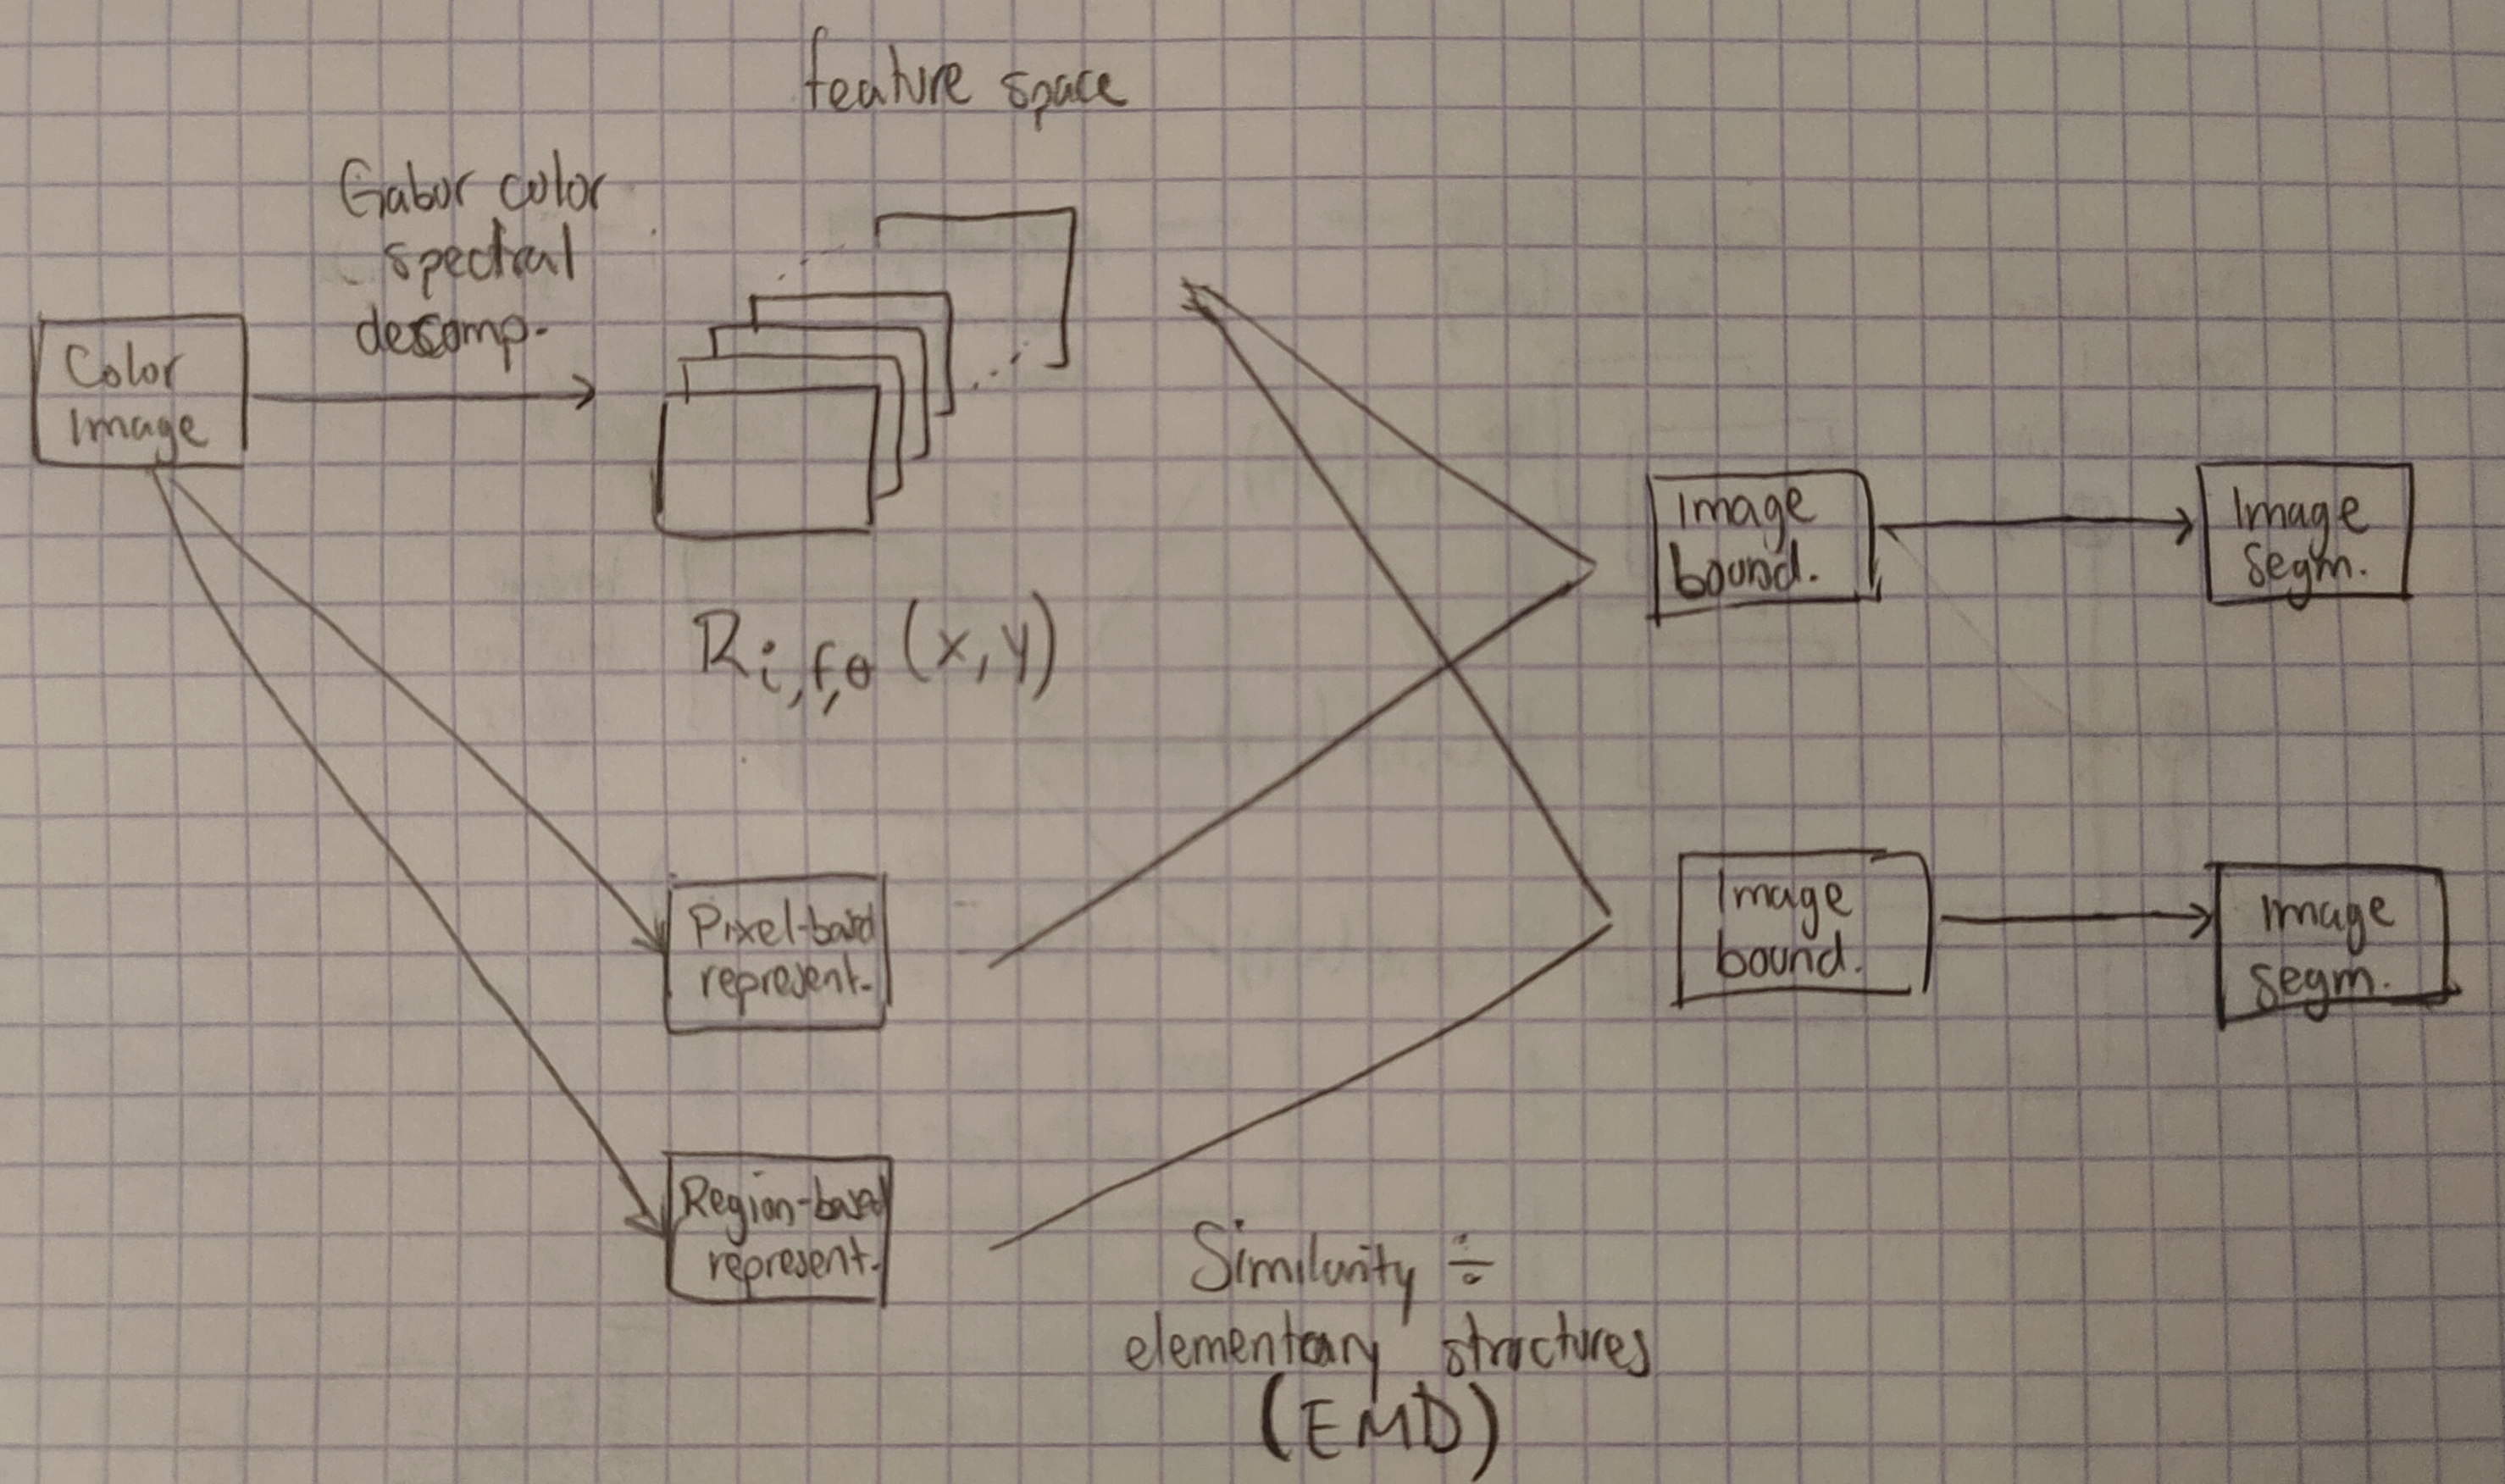
\includegraphics[width=\textwidth]{image_segment_gabor_features}
	\caption{General pipeline for extraction of perceptual imagen boundaties and unsupervised image segmentation.}\label{fig:pipeline_gabor_image_segmentation}
\end{figure}


\section{Image as a graph}

Graphs are historical mathematical structures that have been applied to almost all fields of engineering. Historically, Euler made use of these structures to solve a problem related to the optimal crossing of people across bridges. The success of these structures in fields such as electricity and chemistry, contributed to the creation of a standard nomenclature, giving way to the Graph theory.

Fundamentally, a graph is an useful structure for modeling pairwise relations between objects. In the field of image processing we can find several approaches that make use of graphs. Generally these methods solve a minimization problem. For example, the \textit{minimun spanning tree} approach that aims to find for each pair of nodes, the path with the least weight edges. On the other hand, the \textit{max-flow min-cut} approach aims to maximize flow with the minimum number of cuts in the graph. Both strategies have been successfully applied to the image segmentation problem. Another application example involves the algebraic theory of graphs that studies the spectrum of matrices that represent graphs.

\subsection{Graph notations and definitions}

In this section we introduce some important definitions that will be used throughout the chapter related to graphs and some related structures.

\begin{definition}[Graph]
	A graph $\mathcal{G}$ is defined by the finite sets $(\mathsf{V}, \mathsf{E})$ in which $\mathsf{E} \subset \mathsf{V} \times \mathsf{V}$. The elements of $\mathsf{v} \in \mathsf{V}$ are called \textit{vertices} and the elements of $\mathsf{e} \in \mathsf{E}$ are called edges. Since the edges are a subset of two nodes, we can write them as $\mathsf{e}_{i,j}$ or $\{i,j\} \forall i, j \in V$.
\end{definition}

\begin{definition}[Neighborhood]

\end{definition}

\begin{definition}[Subgraph]

\end{definition}

\begin{definition}[Edge-weighted graph]

\end{definition}

\begin{definition}[Adjacency]

\end{definition}

\begin{definition}[Adjacency matrix]

\end{definition}

\begin{definition}[Node-weighted graph]

\end{definition}

\subsection{Pixel-based representation}


\subsection{Region-based representation}
The term \textit{superpixels} was introduced by (cite Ren and Malik) in 2013. The term superpixels emerge as an oversegmentation process. The motivation lies in the affirmation that pixels are not natural entities, they are consequence of the discrete representation of an image and also that the number of pixels is to high (even in moderate resolutions) making the optimization at pixel level difficult. The superpixels are local coherent and preserve most of the stucture necessary for the segmentation.  

The superpixels technique comes from the oversegmentation techniques; to make the difference between them we can consider the following requeriments:
\begin{enumerate}
 \item Partition. Superpixels should define a partition of the image. They should be disjoint and assign a label to every pixel.
 \item Connectivity. Superpixels represents a connected set of pixels.
 \item Boundary Adherence. Superpixels must preserve image bundaries.
 \item Compactness, Regularity and Smoothness. Superpixels should be compact (closed and bounded), placed regulary and exibit smooth boundaries.
 \item Efficiency. Shuold be generated efficiently
 \item Controllable number of superpixels. The number of superpixels should be controllable.
\end{enumerate}

(Cite David Stutz) propouse a classification for superpixels techniques based on the strategy it follows to obtain the superpixels. Using this classification, superpixels methods currently developed in python lies in the following categories:
\begin{enumerate}
 \item \textbf{Watershed-based.} Based on the watershed algorithm, these methods generally depends on the image pre-processing and the markers setting. 
 \item \textbf{Density-based.} Perform mode-seeking in a computed density image. These methods usually do not offer control over the number of superpixels or their compactness (they are consider as oversegmentation algorithms). 
 \item \textbf{Graph-based.} Treat the image as undirected graph and do a the image partition based on edge-weights  (computed as color differences or similarities).
 \item \textbf{Clustering-based.} Inspired in clissical clustering methods (k-means), these techniques group the pixels from seed pixels using color information, spacial information, and other (such as depth information). The number of superpixels and their compactness is controllable.
\end{enumerate}


\subsubsection{Felzenszwalb's Superpixels}
Graph-based image segmentation techniques generally represent the problem in terms of a graph $G = (V, E)$ where each node $v_i \in V$ corresponds to a pixel in the image, and an edge $(v_i, v_j) \in E$ connects vertices $v_i$ and $v_j$ . A weight $w(v_i, v_j)$ is associated with each edge based on some property of the pixels that it connects, such as their image intensities.

In the graph-based approach, a segmentation $S$ is a partition of $V$ into components such that each component (or region) $C \in S$ corresponds to a connected component in a graph $G = (V, E)$, where $E \subseteq E$. In other words, any segmentation is induced by a subset of the edges in $E$. There are different ways to measure the quality of a segmentation but in general we want the elements in a component to be similar, and elements in different components to be dissimilar. This means that edges between two vertices in the same component should have relatively low weights, and edges between vertices in different components should have higher weights.

This work presents two ways to achieve the segmentacion:

\subsubsection{Grid Graphs}
They define an undirected graph $G = (V, E)$, where each image pixel $p_i$ has a corresponding vertex $vi \in V$. The edge set $E$ is constructed by connecting pairs of pixels that are neighbors in an 8-connected sense (any other local neighborhood could be used). This yields a graph where $m = O(n)$, so the running time of the segmentation algorithm is $O(n log n)$ for $n$ image pixels. We use an edge weight function based on the absolute intensity difference between the pixels connected by an edge, $$w(v_i, v_j) = |I(p_i) - I(p_j)|$$ where $I(p_i)$ isthe intensity of the pixel $p_i$.


\subsubsection{Nearest Neighbor Graphs}
As in the last technique, they use an undirect graph $G = (V, E)$ and the difference lies on the edge weight computation. The weight $w(v_i, v_j)$ of an edge is the distance between the two corresponding points in feature space. They map each pixel to the feature point $(x, y,r, g, b)$, where $(x, y)$ is the location of the pixel in the image and $(r, g, b)$ is the color value of the pixel. They use the $L_2$ (Euclidean) distance between points as the edge weights, although other distance functions are possible.


\subsubsection{Quick Shift and kernel methods for mode seeking}
\begin{description}
 \item \textbf{Kernel methods (Machine Learning). CITE Hoffmann and Campbell } Kernel methods owe their name to the use of kernel functions, which enable them to operate in a high-dimensional, implicit feature space without ever computing the coordinates of the data in that space, but rather by simply computing the inner products between the images of all pairs of data in the feature space. This operation is often computationally cheaper than the explicit computation of the coordinates. This approach is called the \textit{kernel trick}. Kernel functions have been introduced for sequence data, graphs, text, images, as well as vectors.
 
 Kernel is a way of computing the dot product of two vectors $ \mathbf{x}$ and $ \mathbf{y}$ in some (possibly very high dimensional) feature space, which is why kernel functions are sometimes called ``generalized dot product''.

 Suppose we have a mapping $\varphi:\mathbb{R}^{n}\rightarrow \mathbb{R}^{m}$ that brings our vectors in $\mathbb{R}^{n}$ to some feature space $\mathbb{R}^{m}$. Then the dot product of $ \mathbf{x}$ and $ \mathbf{y}$ in this space is $\varphi( \mathbf{x})^{T}\varphi( \mathbf{y})$. A kernel is a function $k$ that corresponds to this dot product, i.e. $k( \mathbf{x}, \mathbf{y})=\varphi( \mathbf{x})^{T}\varphi( \mathbf{y})$.

 \textsl{Example:} Consider a polinomial kernel $k(\mathbf{x},\mathbf{y})=(1+ \mathbf{x}^{T} \mathbf{y})^{2}$ with $\mathbf{x},\mathbf{y} \in \mathbb{R}^{2}$. Assuming that $\mathbf{x}=(x_1, x_2)$ and $\mathbf{y}=(y_1, y_2)$, expanding the expresion: 
 \begin{eqnarray} 
   \nonumber
   k(\mathbf{x},\mathbf{y}) &=& (1+\mathbf{x}^{T}\mathbf{y})^{2}=(1+x_1y_1+x_2y_2)^2 \\ 
   \nonumber
   k(\mathbf{x},\mathbf{y}) &=& 1 + x_1^2y_1^2 + x_2^2y_2^2 + 2x_1y_1 + 2x_2y_2 + 2x_1x_2y_1y_2
 \end{eqnarray}

 We notice that this corresponds to a dot product between the vectors $(1, x_1^2, x_2^2, \sqrt{2}x_1,  \sqrt{2}x_2, \sqrt{2}x_1x_2)$ and $(1, y_1^2, y_2^2, \sqrt{2}y_1,  \sqrt{2}y_2, \sqrt{2}y_1y_2)$. Then  
 \begin{eqnarray} 
   \nonumber
   \varphi(\mathbf{x}) &=& \varphi(x_1, x_2) = (1, x_1^2, x_2^2, \sqrt{2}x_1,  \sqrt{2}x_2, \sqrt{2}x_1x_2) \\ 
   \nonumber
   \varphi(\mathbf{y}) &=& \varphi(y_1, y_2) = (1, y_1^2, y_2^2, \sqrt{2}y_1,  \sqrt{2}y_2, \sqrt{2}y_1y_2)
 \end{eqnarray}

 So the kernel $k(\mathbf{x},\mathbf{y})=(1+ \mathbf{x}^{T} \mathbf{y})^{2} = \varphi(\mathbf{x})^T \varphi(\mathbf{y})$ computes a dot product in 6-dimensional space without explicitly visiting this space. 
 
 Another example is Gaussian kernel $k(\mathbf{x},\mathbf{y})=\exp(- \gamma\parallel \mathbf{x} - \mathbf{y}\parallel^2)$.
 
 \item \textbf{Kernel methods (Statistics).} The term kernel is a term in statistical analysis used to refer to a window function. The term ``kernel'' has several distinct meanings in different branches of statistics. In statistics, kernel density estimation (KDE) is a non-parametric way to estimate the probability density function of a random variable. Kernel density estimation is a fundamental data smoothing problem where inferences about the population are made, based on a finite data sample. In some fields such as signal processing and econometrics it is also termed the Parzen–Rosenblatt window method, after Emanuel Parzen and Murray Rosenblatt, who are usually credited with independently creating it in its current form (WIKI).
 
 
 \item \textbf{Mean shift.} Mean shift is a non-parametric feature-space analysis technique for locating the maxima of a density function, a so-called mode-seeking algorithm (CITE Cheng). Mean shift is a procedure for locating the maxima —the modes— of a density function given discrete data sampled from that function(CITE Cheng). This is an iterative method, and we start with an initial estimate $x$. 
 
 Let a kernel function $K(x_{i}-x)$ be given. This function determines the weight of nearby points for re-estimation of the mean. Typically a Gaussian kernel on the distance to the current estimate is used, $K(x_{i}-x)=e^{-c \parallel x_{i}-x \parallel ^{2}}$. The weighted mean of the density in the window determined by $K$ is $$ m(x) = \frac{ \sum_{x_i \in N(x)} K(x_i - x) x_i } {\sum_{x_i \in N(x)} K(x_i - x)}$$ where $N(x)$ is the neighborhood of $x$, a set of points for which $K(x_i) \neq 0$.
 
 The difference $m(x)-x$ is called mean shift in Fukunaga and Hostetler (CITE). The mean-shift algorithm now sets $x \leftarrow m(x)$, and repeats the estimation until $m(x)$ converges.
 
 \item \textbf{Medoids.} Are representative objects of a data set or a cluster with a data set whose average dissimilarity to all the objects in the cluster is minimal. Medoids are similar in concept to means or centroids, but medoids are always restricted to be members of the data set. Medoids are most commonly used on data when a mean or centroid cannot be defined, such as graphs. They are also used in contexts where the centroid is not representative of the dataset like in images and 3-D trajectories and gene expression (where while the data is sparse, the medoid need not be). These are also of interest while wanting to find a representative using some distance other than squared euclidean distance.
 
 \item \textbf{Medoid shift (CITE Sheikh).} Medoid shift is a modification of mean shift, the main difference: Meanshift selects the location that minimizes this function exactly while Medoidshift selects the data point that best minimizes it (medoid). Another difference is that the data space $X$ may be non-Euclidian.
\end{description}

Taking the above concepts, the Quick Shift method simply propose moves each point $x_i$ to the nearest neighbor for which there is an increment of the density $P(x)$ (CITE Vedaldi).  


\subsubsection{Compact watershed segmentation of gradient images}
This method retakes the watershed segmentation proposed by (CITE Meyer). Originally, the watershed method is an over segmentation technique, i.e., one can control the number of regions by means of the number of markers but we cannot control its compactness.  In this context, high compactness means that the superpixels are of approximately equal size and more or less regularly shaped in the absence of strong image gradients (e.g. like a recangle or a circle). The method proposed by (CITE Neubert) upgrades the original algorithm adding the compactness. 

At base, the algorithm is an implemetation of the OpenCv funtion ``watershed'' whichs implements a seeded watershed segmentation (also called marker controlled watershed). The seeds are externally provided to the algorithm, e.g. as local gradient minima or for superpixel-like segmentation on a uniform grid. The seeds grow iteratively pixel by pixel until they reach a border to the segment around another seed. These borders form the watersheds. The next seed to expand by one pixel is chosen based on a distance function. In the OpenCV implementation, this distance function only incorporates the intensity or color value of the pixels. To influence the compactness of the segmentation, they propose the simple extension of incorporating the distance to the seed point as well.


\subsubsection{SLIC superpixels}
This algorithm simply performs K-means in the 5-d space of color information and image location and is therefore closely related to quickshift. As the clustering method is simpler, it is very efficient. It is essential for this algorithm to work in Lab color space to obtain good results

\subsubsection{Superpixels techniques comparison}

\section{Perceptual image boundaries}
\subsection{Earth Mover's Distance for non-normalized distributions}

\subsection{Image segmentation based on image gradients}
\subsubsection{MST threshold graph-cut}
This method is based on the graph cut using a threshold value. However, the choice of this threshold value is not always obvious, and this value may differ for each image.
We propose obtaining a threshold value by fitting a probability density function to the values of the egdes of the image graph. Our hypothesis is that the areas with the same color and / or texture information behave as flat areas in the generated feature space, therefore those edges that connect these areas behave as outliers within the probability function. Under this principle, we can propose a cut at some quantile level of the distribution, for example, to 90\%.

In addition, to increase the visibility of outliers, we reduce the number of edges by applying the distribution of the function on the minimun spaning tree (MST) of the k-nn graph.

%\begin{figure}[!ht]
%\centering
%\includegraphics[width=0.4\textwidth]{cow_mst_weight_dist.png} \caption{Weight distribution of the edges of the MST of an image.  On the values we fit a log-norm probability function}
%\end{figure}\label{fig:gradient_computation_diagram}
%
%\begin{tabular}{ccc}
%\includegraphics[width=0.33\textwidth]{8068_graphcut_result.png}  & \includegraphics[width=0.33\textwidth]{15062_graphcut_result.png} & \includegraphics[width=0.33\textwidth]{48017_graphcut_result.png}\\
%\end{tabular}


\subsubsection{Spectral clustering}
To apply this segmentation method, we obtain a affinity matrix from the adjacency matrix generated from the connections of the k-nn graph. The normalization of the affinity matrix is a prerequisite for achieving image segmentation. To achieve this, we apply a global normalization with a sigma parameter.

%\begin{tabular}{ccc}
%\includegraphics[width=0.33\textwidth]{8068_spec_result.png}  & \includegraphics[width=0.33\textwidth]{15062_spec_result.png} & \includegraphics[width=0.33\textwidth]{48017_spec_result.png}\\
%\end{tabular}

\subsubsection{Normalized graph-cut}
In the same way as the spectral clustering method, the normalized slicing method uses a normalized affinity matrix. The differences between these two methods lie in the speed of calculation and the need to define a number of clusters. In the case of spectral clustering, the calculation time is less, however, it is necessary to give an estimated number of regions to find.

\subsubsection{Gradient-based segmentation comparison}

Taking into account the great variety of techniques, models, strategies and their respective parameters used in this work, we wanted to cover the widest possible range of variables in our tests.

Therefore, to evaluate the learning of the importance of color and texture and to have a qualitative score, we calculated the F-score using the segmentation results of each method mentioned above. The calculation of such a score can be done individually, that is, by image, however, we collect the set of scores from the BSD test subset and use them in some box plots. These graphs first show the precision and recall of each method, but it also allows us to see which Gabor space configuration gives the best results.


%\includegraphics[width=\textwidth]{Thr_graphcut_Fscores_log_mst_boxplot_pred_linreg.png}  \\
%Scores using the gradients predicted by the linear regression model (LinReg) and the Threshold graph cut method\\
%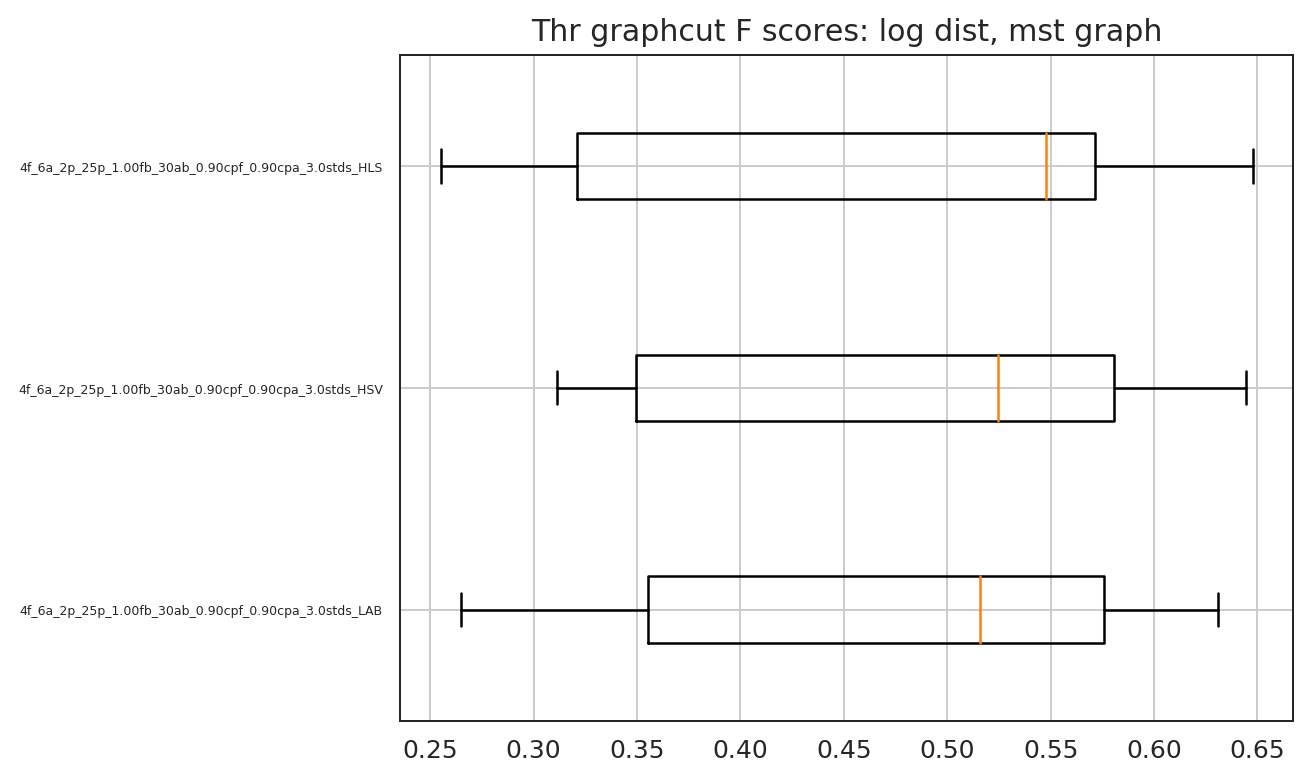
\includegraphics[width=\textwidth]{Thr_graphcut_Fscores_log_mst_boxplot.png} \\
%Scores using the sum of the computed gradients and the Threshold graph cut method\\
%\includegraphics[width=\textwidth]{Spectral_clustering_Fscores_global_complete_boxplot_pred_linreg.png} \\
%Scores using the gradients predicted by the linear regression model (LinReg) and the Spectral Clustering method\\
%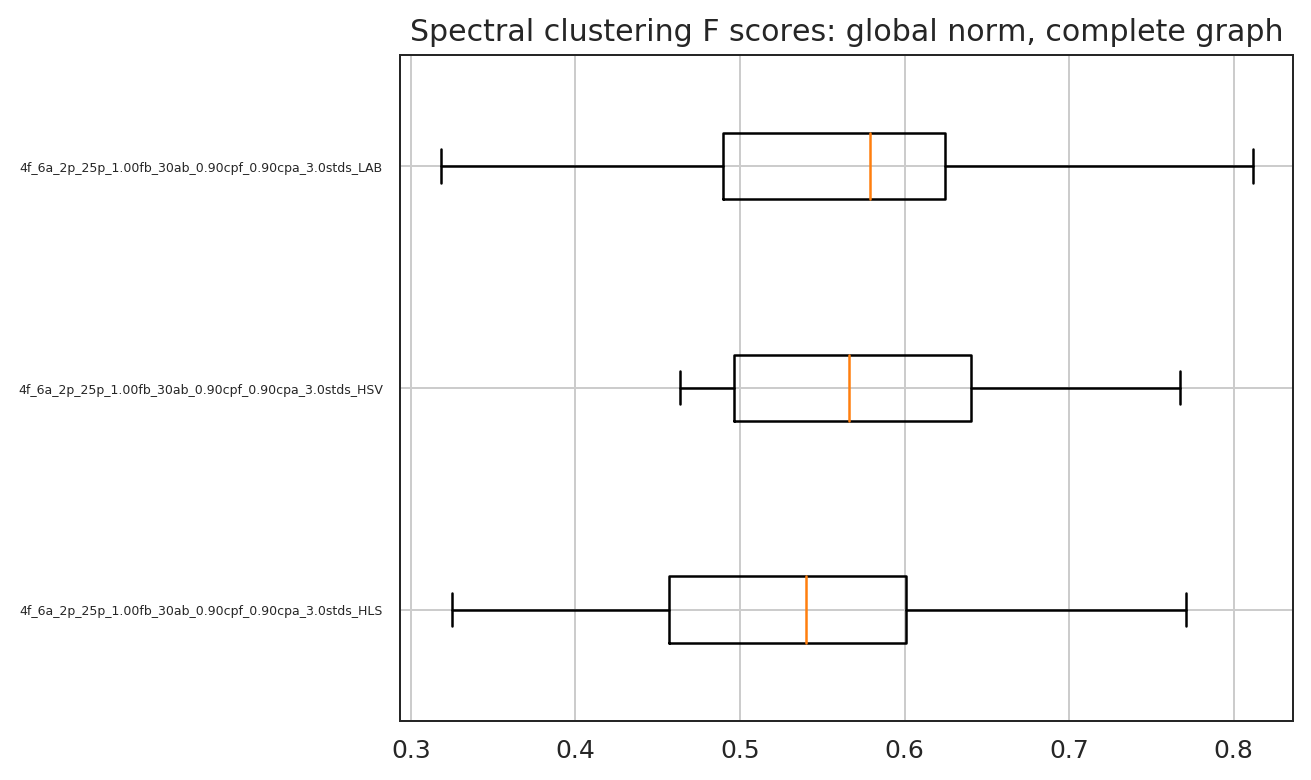
\includegraphics[width=\textwidth]{Spectral_clustering_Fscores_global_complete_boxplot.png}\\
%Scores using the sum of the computed gradients and the Spectral Clustering method\\

\section{Perceptual image segmentation}
\subsection{Hierarchical watershed}
\subsection{Interactive image segmentation}



\section{Comparison with the state of the art}
\subsection{Scores}
\subsection{Results}


\section{Importance of color and texture in image segmentation}


\section{Conclusions}
